\section{Discussione dei Modelli}\cite{STATISTICALLEARNING}

In questa sezione si discuteranno quali motivi mi hanno spinto a scegliere i modelli utilizzati e come essi funzionano.
\subsection{Scelta dei Modelli}

Ho voluto scegliere algoritmi di classificazione poichè, riferendomi all'EDA (subsection. \ref{ssec:EDA}), in particolare alla matrice di correlazione, fig.\ref{fig:matr_corr}, non vi è nessuna feature correlata all'uscita in modo lineare e quindi non ho potuto applicare nessun modello di regressione lineare. Inoltre le uscite sono valori discreti, quindi perfetti per una classificazione.
Per la mia classificazione ho voluto utilizzare due modelli:
\begin{itemize}
    \item K-Nearest Neighbors
    \item Decision Tree
\end{itemize}
La scelta del primo è dovuta al fatto che è un algoritmo semplice e, sebbene all'aumentare dei dati il KNN sia decisamente lento per le ragioni sotto riportate, per la mia mole di dati è abbastanza veloce. Non c'è inoltre bisogno di costruire un vero e proprio modello come nel caso di altri algoritmi.
\break La scelta del secondo modello, il Decision Tree, è dovuto al fatto che è molto veloce nel classificare nuovi dati. Per giunta, la visualizzazione dell'albero decisionale è di facile comprensione sopratutto in ambito medico. Quindi un dottore potrebbe facilemente interpretare il modello e classificare il tipo di fibrosi di un nuovo paziente. 

\subsection{K-Nearest Neighbor}

Il principio del KNN è diverso dagli altri algoritmi di apprendimento. Infatti esso non scarta il training set una volta che il modello è costruito, mantenendo tutto il training set in memoria. L'algoritmo, una volta che vede un nuovo sample x, trova i "k" training samples più vicini a x e ritorna la label maggioritaria tra questi samples, ovvero per i casi di regressione la media, per i casi di classificazione la moda. La vicinanza di due samples è data da una funzione di distanza. Essa può essere di diversi tipi, come per esempio:
\begin{itemize}
    \item Distanza Euclidea
    \item Distanza di Chebychev
    \item Distanza di Mahanattan
\end{itemize}
La distanza euclidea, con \begin{math}q\end{math} indicante un punto in molteplici dimensioni, può essere definita come:
\begin{equation}
    d(q^{i},q^{l})=\sqrt{\sum_{j=1}^{p}(q_{j}^{(i)}-q_{j}^{(l)})^{2}}
\end{equation}
Il numero k di vicini è un iperparametro e per questo dev'essere "settato" correttamente, altrimenti con k molto piccoli o troppo grandi si potrebbe avere una predizione molto instabile. Se k aumenta, si diminuisce il rumore che compromette la giusta classificazione, tuttavia se k diminuisce la classificazione non è facilmente determinabile.  

\begin{figure}[H]
    \centering
    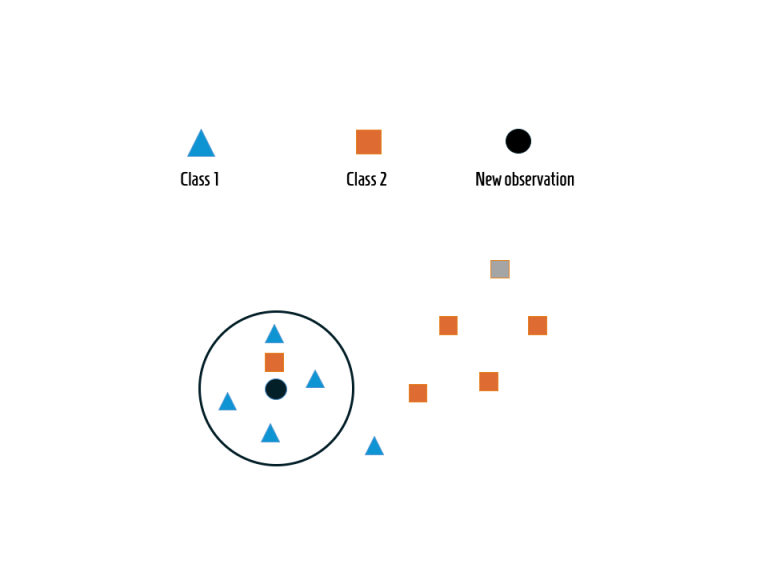
\includegraphics[width=0.65\columnwidth]{figures/k-nearest-neighbor-768x576.png}
    \caption{KNN}
    \label{fig:target}
\end{figure}

\subsection{Decision Tree}

Il Decision tree o albero decisionale è un algoritmo appartenente alla famiglia dei modelli supervisionati. Esistono due tipo di Alberi, quelli per la classificazione e quelli per la regressione. Il discriminante è che il primo utilizza dati discreti come nel mio caso, il secondo valori continui.
Un albero è costuituito da 3 elementi cardine:
\begin{itemize}
    \item Nodi: testano il valore di un certo attributo
    \item Foglie: Sono i nodi terminali, che predicono il risultato
    \item Rami: sono i collegamaneti tra i risultati dei test e il nodo successivo, o foglia
\end{itemize}
I dati sono continuamente suddivisi in base ad un certo parametro. Infatti in questo grafo aciclico (l'albero) uno specifico vettore feature viene esaminato e, se il valore della feature è sotto una certa soglia, viene seguito il ramo di sinistra, altrimenti quello di destra. Questo algoritmo, come fa supporre il nome, impara attraverso i dati che ha a disposizione.
\newline Vengono seguite le seguenti regole:
\begin{itemize}
    \item Seleziona un test per il nodo radice e crea un branch per ogni possibile risultato di questo test
    \item Divide le istanze in sottoinsiemi, uno per ogni ramo che si estende dal nodo
    \item Ripete in modo ricorsivo, usando solo istanze cha raggiungono il ramo
    \item Ferma la ricorsione per un ramo se tutte le sue instanze hanno lo stesso output
\end{itemize}
Quello che si cerca di effetture, per evitare di considerare ogni possibile partizione dello spazio delle features, è usare il \textbf{recursive binary splitting}, ovvero selezionare il cutpoint e le features che portano alla maggiore impurità dei nodi. Un nodo è definito \textbf{puro} quando tutti i samples nello stesso "split" hanno lo stesso valore di uscita. Come misurare l'impurità di un nodo? Attraverso l'indice di Gini, cioè un valore tra 0 e 1 in cui il valore 0 indica che tutti gli elementi appartengono ad una specifica classe mentre 1 evidenzia che gli elementi sono distribuiti in modo totalmente casuale in varie classi. Dunque un indice di Gini che vale 0.5 suggerisce che gli elementi sono equamente distribuiti nelle varie classi.
\newline Purtroppo però i Decision Tree sono soggetti all'overfitting, ovvero si adatta fortemente ad uno specifico training set e questo comporta a predire valori mai visti in modo completamente anomalo. Inoltre minimi cambiamenti dei dati di training possono comportare una logica di decisione completamente diversa.
\begin{figure}[H]
    \centering
    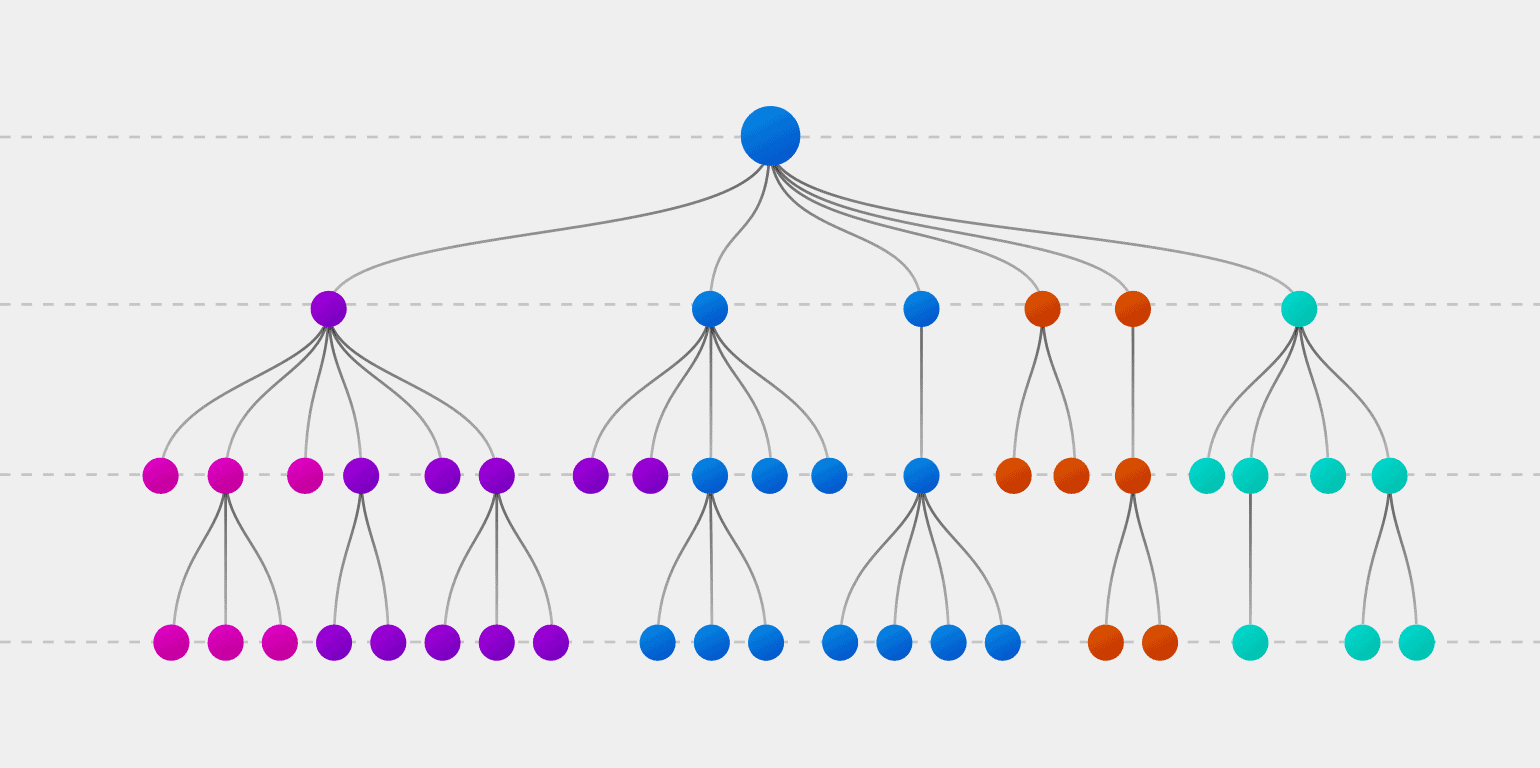
\includegraphics[width=0.65\columnwidth]{figures/Decision-Trees.png}
    \caption{Albero decisionale}
    \label{fig:target}
\end{figure}